\documentclass{article}
\usepackage{amsmath}
\usepackage{amssymb}
\usepackage{array}
\usepackage{booktabs}
\usepackage{makecell}
\usepackage{multirow}
\usepackage{enumitem}
\usepackage{diagbox}
\usepackage{tabularx}
\usepackage{graphicx}
\usepackage{multirow}
\usepackage[top=3cm,bottom=2cm,left=2cm,right=2cm]{geometry} % 页边距
\title{Software System Design-Architecture\\Assignment 3\\C4 System Architecture Design}
\author{4 people}

\begin{document}
	\maketitle
	\newpage
	\section{Deploying ADD method in C4 Design}
	\subsection{Important Non-functional Requirements}
	The important non-functional requirements we identified are listed bellow:
	\begin{itemize}
		\item {Availability}
		\item {Performance}
		\item {Modification}
		\item {Scalability}
		\item {Interoperability}
		\item {Consistency}
		\item {Integrity}
		\item {Usability}
	\end{itemize}
	The constrains we identified are listed bellow:

	\begin{itemize}
		\item No persistent data caching on the agent workstations to limit the implications of local failures.
		\item No DBs at office locations.
		\item No administrators at local offices.
		\item No maintenance down-time.
		\item The middle layer server cluster tuned for performance.
		\item The back end tuned for DB performance.
		\item Well engineered operations architecture.
		\item High availability cannot be achieved by utilizing fault-tolerant hardware (this option is not
		economically viable).
	\end{itemize}
	The scenarios are listed as following:

	\begin{center}
		\begin{table}[!htb]
		\begin{tabular}{ccc}
		\toprule  
		Portion of Scenario & Possible Values\\
		\midrule 
		Source & End users and internal systems.\\
		Stimulus & Failure and fault: Service off-line, error, \\
		& crash ans so on.\\
		Artifact & Back up, spare, communication channels.\\
		Environment & Runtime, startup and shutdown, in-service.\\
		Response & Able to response for many requests at the \\
		& same time.\\
		& Detect the fault. \\
		& Recover from the fault. \\
		& Prevent the fault. \\		
		Response Measure & Availability percentage(e.g. 99\%) \\
		& Time to be back to service after an error occured \\
		& Time to detect a failure \\
		\bottomrule
		\end{tabular}
		\caption{Availability Scenario}
		\end{table}
	\end{center}

	\begin{center}
		\begin{table}[!htb]
		\begin{tabular}{ccc}
		\toprule  
		Portion of Scenario & Possible Values\\
		\midrule 
		Source & End users and internal systems.\\
		Stimulus & Many requests come at the same time.\\
		Artifact & A waiting queue or something could  \\
		& caching the request temporarily. A mechanism  \\
		& to serve the request after a short interval.\\
		Environment & In-service. \\
		Response & The C4 should be able to deal with a large \\
		& bunchs of requests. And after a short interval, the \\
		& request would be processed.\\
		Response Measure & The time taken to serve every request.\\
		& The lateness of the processing.\\
		\bottomrule
		\end{tabular}
		\caption{Performance Scenario}
		\end{table}
	\end{center}

	\begin{center}
		\begin{table}[!htb]
		\begin{tabular}{ccc}
		\toprule  
		Portion of Scenario & Possible Values\\
		\midrule 
		Source & Developers.\\
		Stimulus & Add some interface to fit for a new requirement.\\
		& Need to improve the system to cater for the increasing \\
		& demand resulted from the rapid growing users.\\
		Artifact & Code, interface, components and so on.\\
		Environment & Runtime or off-line, in the design \\
		& process or in the maintaining process\\
		Response & Make the modifications.\\
		Response Measure & The effort, time and money taken\\
		& to implement such requirement.\\
		\bottomrule
		\end{tabular}
		\caption{Modification Scenario}
		\end{table}
	\end{center}

	\begin{center}
		\begin{table}[!htb]
		\begin{tabular}{ccc}
		\toprule  
		Portion of Scenario & Possible Values\\
		\midrule 
		Source & System customers.\\
		Stimulus & More system customers or requests.\\
		Artifact & Server cluster.\\
		Environment & In the process of normal service provision of the system, \\
		& the customers of the system grow \\
		& from a small group to a huge network, \\
		& or the number of customer requests grows rapidly.\\
		Response & Scaling horizontally by adding servers, \\
		& the cluster load is forwarded to the newly added servers.\\
		Response Measure & Increase the workload of new servers; \\
		& The ratio of system throughput improvement to \\
		& the number of increased servers; \\
		& The time the horizontal expansion takes effect, etc.\\
		\bottomrule
		\end{tabular}
		\caption{Scalability Scenario}
		\end{table}
	\end{center}

	\begin{center}
		\begin{table}[!htb]
		\begin{tabular}{ccc}
		\toprule  
		Portion of Scenario & Possible Values\\
		\midrule 
		Source & Communication between systems and outside systems.\\
		Stimulus & The system initiates data manipulation requests from other systems \\
		& or processes data manipulation responses from other systems.\\
		Artifact & Protocol module, \\
		& Asynchronous communication module (including message queue).\\
		Environment & During normal operation, the system \\
		& needs to request relevant data from other systems \\
		& or persist the data generated by the system to other systems.\\
		Response & When a system makes a request to another system, \\
		& it encapsulates the request event or data into a message \\
		& in a predefined format. When processing the response of other systems, \\
		& the message in the predetermined format is parsed \\
		& into the event or data format within the system. \\
		& In synchronous communication, the order of request events \\
		& is guaranteed to be executed through synchronous message queue. \\
		& After issuing the request, the system should wait \\
		& for the response from other systems and then carry out subsequent operations. \\
		& In asynchronous communication, after the system issues a request, \\
		& it continues to carry out subsequent operations without waiting for the response. \\
		& When the response messages of other systems reach the system, \\
		& they will be cached in the message queue. \\
		& The asynchronous communication module periodically checks the message queue \\
		& and processes the relevant messages to be processed.\\
		Response Measure & The proportion of communicating messages \\
		& that are properly processed; The proportion of messages \\
		& communicated being correctly rejected; Communication delay; \\
		& Average number of message transfers per communication \\
		& (encoding efficiency); Communication throughput.\\
		\bottomrule
		\end{tabular}
		\caption{Interoperability Scenario}
		\end{table}
	\end{center}

	\begin{center}
		\begin{table}[!htb]
		\begin{tabular}{ccc}
		\toprule  
		Portion of Scenario & Possible Values\\
		\midrule 
		Source & The system processes multiple concurrent tasks simultaneously.\\
		Stimulus & There are multiple customers operating on \\
		& the same system resource at the same time, \\
		& or the same customer recovering the last interrupted \\
		& configuration request transaction.\\
		Artifact & The whole system. \\
		Environment & In the process of normal service provision of the system, \\
		& multiple customers will request configuration of the same resource. \\
		& At the same time, the system provides the service function of \\
		& configuring request interruption and persistence context preservation.\\
		Response & The system resource locks the first customer operation \\
		& until the lock is released after the operation is completed, \\
		& during which the operation request of other customers \\
		& will be rejected and fail. When the customer is interrupted during the configuration request, the system saves the processing context, and resumes the context saved during the interruption when the same customer requests again.\\
		Response Measure & The time cost of context saving and recovery; Granularity of distributed locks (the range of resources affected by locking); The average number of successful lock attempts on system resources.\\
		\bottomrule
		\end{tabular}
		\caption{Data Consistency Scenario}
		\end{table}
	\end{center}

	\begin{center}
		\begin{table}[!htb]
		\begin{tabular}{ccc}
		\toprule  
		Portion of Scenario & Possible Values\\
		\midrule 
		Source 				& The client is going to request related information \\
							& from the target server , usually the important \\
							& personal infomation\\
		Stimulus 			& The infomation sends back to the client\\
		Artifact 			& Client PC	\\
		Environment 		& Query from DB , server cache and Request queue\\
		Response 			& The server has to fetch the user request and \\
							& conduct the related query from the data source,\\
							& with the maintenance of the data integrity. \\
							& To maintain the data integrity , the server \\
							& should checkout whether the data has the \\
							& latest version and no other conflict \\
							& writing conduction is on going.\\
		Response Measure 	& The data sent back to the user\\
							& has to be 100 percents integrity.\\

		\bottomrule
		\end{tabular}
		\caption{Integrity Scenario}
		\end{table}
	\end{center}
	
	\begin{center}
		\begin{table}[!htb]
		\begin{tabular}{ccc}
		\toprule  
		Portion of Scenario & Possible Values\\
		\midrule 
		Source 				& More customer load push on the system\\
		Stimulus 			& More than five thousand of user are using the system\\
		Artifact 			& Master server , keeper\\
		Environment 		& Network connection , agent requests \\
		Response 			& The server should detect the specific \\
							& server that is overloaded, \\
							& and reallocate the request to other leisure node;\\
							& The keeper should arrange the request queue to ensure \\
							& the synchronize the data flow in the process ,\\
							& ensuring the data is always correct.\\
		Response Measure 	& Load balance , horizontal expansion and request queue \\
							& to resolve the high concurrency\\


		\bottomrule
		\end{tabular}
		\caption{Availability Scenario}
		\end{table}
	\end{center}

	\begin{center}
		\begin{table}[!htb]
		\begin{tabular}{ccc}
		\toprule  
		Portion of Scenario & Possible Values\\
		\midrule 
		Source 				& One agent somehow choose to save the session and \\
							& return back to continue the session.\\
		Stimulus 			& The system is going to save the context of the \\
							& current session of agents.\\
		Artifact 			& A session which represents the current \\
							& state of both agents' information , \\
							& session attributes and so on.\\
		Environment 		& keeper \\
		Response 			& The keeper reply the saving request \\
							& and put the session information to the \\
							& base storage in keeper's cluster , \\
							& and set back the session identification to agents.\\
		Response Measure 	& Set up local storage which is responsible of saving sessions\\
							&  in the server of keeper and  \\
							& arrange the location of the storage.\\
		\bottomrule
		\end{tabular}
		\caption{Usability Scenario}
		\end{table}
	\end{center}
	
\newpage

	\subsection{Records of ADD iterations}
		\subsubsection{Iteration 1}
			\paragraph{Chosen element} the whole system.
			\paragraph{Chosen ASR}
			\begin{enumerate}
			\item Near 7x24 availability.
			\item It should allow for "leaner" growth and should be able to grow at a rapid rate.
			\end{enumerate}
			\paragraph{Design Concerns} high availability, high scalability.
			\paragraph{Alternative Patterns}
			\begin{center}
				\begin{tabular}{|c|c|}
					\hline
					Design Concerns & subordinate Concerns\\
					\hline 
					% \multirow{rows}{width}{text}
					% \multirow{2}*{Availability \& Scalability} & broker\\
					% \cline{2-2}
					% ~ & redundant broker\\
					Availability \& Scalability & broker\\
					\hline
				\end{tabular}
			\end{center}
			\paragraph{Select patterns}
			\subparagraph{Alternative broker tactics}
			Discriminating parameters:\\
			\begin{itemize}
				\item complexity
				\item fault-tolerance
			\end{itemize}
			\begin{center}
				\begin{tabular}{|c|c|c|}
					\hline
					pattern name & complexity & fault-tolerance\\
					\hline
					broker& low& low\\
					\hline
					redundant broker& high& high\\
					\hline
				\end{tabular}
			\end{center}
			\subparagraph{Chosen pattern} 
			redundant broker
			\subparagraph{Reason} 
			Added broker can help manage server nodes and easily achieve high availability. But the business background goal that the system can handle requests simultaneously with highly growing customers will implies high pressure on the broker. Redundant broker is adopted for data backup quick switch in emergency condition. 

			% \subparagraph{Alternative scalability tactics}
			% Discriminating parameters:\\
			% \begin{itemize}
			% 	\item a
			% 	\item b
			% \end{itemize}
			% \begin{center}
			% 	\begin{tabular}{|c|c|c|}
			% 		\hline
			% 		pattern name & complexity & fault-tolerance\\
			% 		\hline
			% 		broker& low& low\\
			% 		\hline
			% 		redundant broker& high& high\\
			% 		\hline
			% 	\end{tabular}
			% \end{center}
			% \subparagraph{Chosen pattern} 
			% redundant broker
			% \subparagraph{Reason} 
			% Added broker can help manage server nodes and easily achieve high availability. But the business background goal that the system can handle requests simultaneously with highly growing customers will implies high pressure on the broker. Redundant broker is adopted for data backup quick switch in emergency condition. 


		\subsubsection{Iteration 2}
		Chosen ASR: 
		1.can handle a batch of requests simultaneously and can support multiple agents.
		2.should manage a big cluster/allow for "leaner" growth
		3.near 7x24 availability.
		4.identification, monitoring, and elimination of processing bottle-necks
		Design Concerns:
		Master Self-test
		Real-time Server Detection:Health detection
		Server Recovery: Fast restart, Transparency to PC, Data recovery
		Service Registry: Locating nodes, Resource allocation, Resource collection, Horizontal extension

		Candidate architecture patterns/tactics:
		Master Self-test:
			pattern name, detection latency
			Hot spare, <100ms
			Warm spare, >1s
			Cold spare, >5s


		\subparagraph{Health detection}
		Discriminating parameters:\\
		\begin{itemize}
			\item communication pressure
			\item storage pressure
			\item report threshold
			\item rate
			\item transparent to PC
		\end{itemize}
		\begin{center}
			\begin{tabular}{|c|c|c|c|c|c|}
				\hline
				pattern name & communication pressure & storage pressure & report threshold & rate & transparent to PC\\
				\hline
				Loading table & high & high & no & controllable& yes\\
				\hline
				Server warning & low & low & controllable & up to context & almost\\
				\hline
				PC warning & no & no & uncontrollable & up to context & not\\
				\hline
			\end{tabular}
		\end{center}
		
		Fast restart:
			...
		
		Transparency to PC:
			...
		
		Data Recovery:
			...
		
		Service Registry:
			...https://docs.qq.com/doc/DVU9YdkxKZWJTQ0VY
		
		Locating nodes:
			... 

		Resource allocation:
			...

		Resource collection:
			... 

		Horizontal extension:
			...

		Chosen pattern/tactics:
			Master Self-test:
				Hot spare
			Chosen reason: 

			Health detection:
				Loading table
			
			Fast restart:
				
			
			Transparency to PC:
				...
			
			Data Recovery:
				...
			
			Service Registry:
				...
			
			Locating nodes:
				... 

			Resource allocation:
				...

			Resource collection:
				... 

			Horizontal extension:
				...
		
		\subsubsection{Iteration 3}
		Chosen ASR: 
		1. should resolve and merge event conflicts.
		2. able to maintain connection context
		Design Concerns: 
		Resource Consistency Maintenance: Detect data conflicts, Restore inconsistent data, Prevent data conflicts
		Context Recovery: Storage and restorage, Fault detection

		Candidate architecture patterns/tactics:
		Detect data conflicts:
			pattern name, time consumption, detection lateness
			Data relation model, high, low
			Multiple backups comparison, low, high
		
		Restore inconsistent data:
			pattern name, probability for losing data, time consumption
			Roll back, middle, low
			Multiple backups restore, low, high
		
		Prevent data conflicts:
			pattern name, difficulty, reliability
			Transaction, hard, high
			Retry, simple, efficient to conditional conflicts but not internal ones

		Storage and restore:
			pattern name
			context storage

		Fault detection:
			pattern name, able to detect fault
			Redundant backup, yes
			No redundant, no
		
		
		Chosen patterns/tactics:
		Detect data conflicts:Multiple backups comparison
		reason: There are multiple servers in keeper module, resulting to natural achievement of multiple backups.   

		Restore inconsistent data: Multiple backups restore
		reason: The same as above.

		Prevent data conflicts: Transaction
		reason: Retry is unreliable.

		Fault detection: Redundant backup
		reason: Redundant backups are necessary.

		\subsubsection{Iteration 4}
		Chosen ASR: 
		1.can communicate with other systems asynchronously.
		2.can well communicate.
		Design Concerns:
		1.Asynchronous communication: Asynchronous requests, time-out detection
		2.Good communication: Satisfy interface, Reduce messages.

		Candidate architecture patterns/tactics:
		Asynchronous requests:
			pattern name, priority, customization, complexity
			Message queue, no, no, low
			Scheduling, yes, yes, high
		
		Time-out detection:
			pattern name, report rate, complexity
			Retry, 0.5s, middle
			Report, 0.1s, low
		
		Satisfy interface:
			pattern name, has performance bottle-neck, extra pressure
			Distributed protocol, low, no, no
			Special intensive protocol, high, yes, on special module
			Master centric protocol, high, yes, on master
		
		Reduce messages:
			pattern name
			local storage
		
		Chosen patterns/tactics:
		Asynchronous requests:Scheduling
		reason: Priority is needed.

		Time-out detection:
		Time-out detection: Report
		reason: retry is not necessary.

		Satisfy interface: Distributed protocol
		reason: Introducing special will lead to a series problems about data consistency. Cannot bring more pressure to Master module which is the main entrance of the system.


		
		

	\section{Final Software Architecture Documentation}
	\subsection{Documentation Roadmap}
	\subsubsection{Scope and summary}
	This documentation is built for presence, explanation and analysis of the architecture of Call Center Customer Care(C4) System, which will be employed by ** US telecommunication company. In this documentation, expression and illustration of modules and theirs relationship will be covered, but not all functions of the system are included.
	\subsubsection{How the documentation is organized}
	catalog
	\subsubsection{View overview}
	4 Views are employed to illustrate the architecture, including:\\  
	Decomposition view: The elements of this view are static modules, and connections illustrate their relationship.\\  
	Shared-data view: We using this view to express how important data are shared and protected from inconsistency resulted by business events....  \\
	Deployment view: This view also illustrate different parts of the software. Distinguished with module view, it focuses on the runtime status rather than the static status of the system.\\
	All of the three views are following the standard UML specification.
	\subsubsection{How stakeholders can use this documentation}
	Stakeholders can use the system to obtain the architectural organization of the entire C4 system, and the way of association with the C4 system and other systems.
	Through the refined ASR design and tactic, pattern acquisition architecture evaluation program.\\
	In addition, based on the system architecture design, Stacksholders can give a preliminary architectural evaluation to facilitate the improvement and maintenance of the subsequent product realization phase.
	Relevant views are given in the testing and deployment of the product, and Stackholders can get the specific ideas of the view design to help Stackeholers understand the system.\\
	\subsection{How a View Is Documented}
	Refer to the view template

	\subsection{System Overview}
	System functions, users, important background, constrains.
	\paragraph{System functions}
	The system mainly supports communication with customers, including requesting new services, changing existing service configurations, or reporting problems.
	\paragraph{Users}
	Users of the system include office agents, auditors, system administrators, operations and maintenance personnel, and infrastructure support personnel.
	\paragraph{Important Background}
	The initial use of the system is for a small group of customers, but it is possible that with the growth of the business, the customer base will develop into a large network; Meanwhile, the system needs to communicate and interact with external systems (NOSS, Enterprise DBs, downstream subsystems, etc.) to complete the whole business process. System services are always online and need to provide near 7*24 hour accessibility.
	\paragraph{Constrains}
	Due to the high traffic and high concurrency of system services, the system needs to provide a good operation and maintenance structure for end users. The database cannot be deployed to the agent's office; In consideration of economic cost, expensive hardware cannot be used to realize fault tolerance.
	
	\subsection{Views}
		\subsubsection{Decomposition View} 
			\paragraph{Section 1: The Primary Presentation}
			\begin{center}
			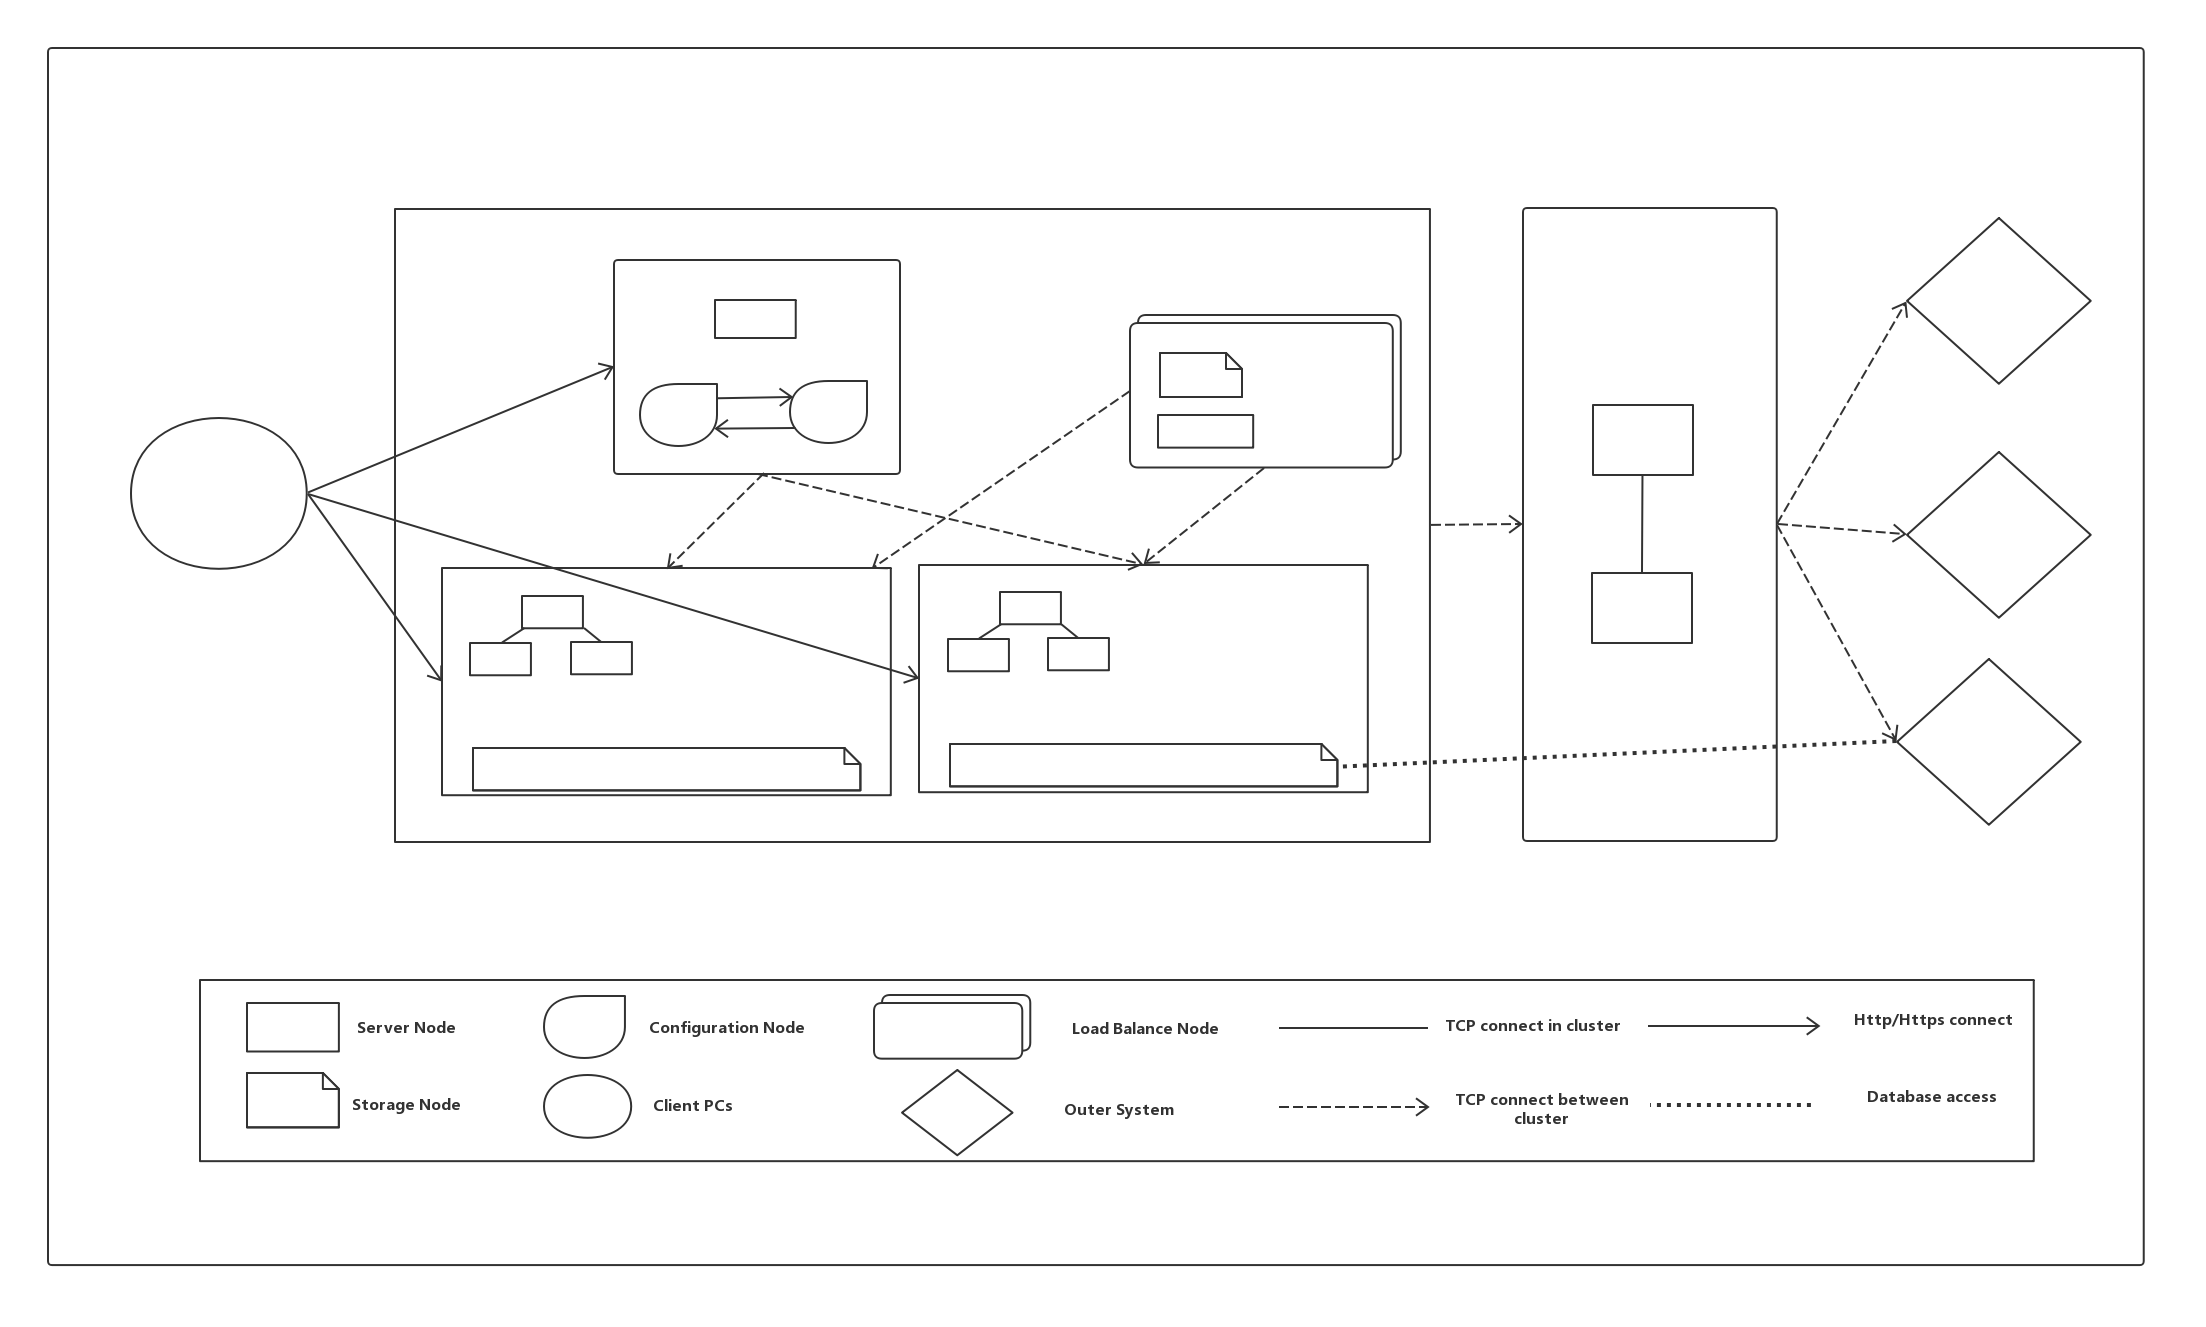
\includegraphics[scale=0.15]{decom_section1.png}
			\end{center}
			\paragraph{Section 2: The Element Catalog}
			The C4 system is consisted of these important sub-module to decompose:  master node , normal server node , storage node , configuration node , load balance node. To resolve the normal phone request (contains the sync-request and async-request) , the normal server nodes are responsible to tackle the service from customers. Moreover , the storage nodes have to save the current session , cache the query on DB , and other cache to the locks . Load balance node has to detect the load in the whole system , and reschedule the load accordingly. 
			\paragraph{Section 3: Context Diagram}
			\begin{center}
			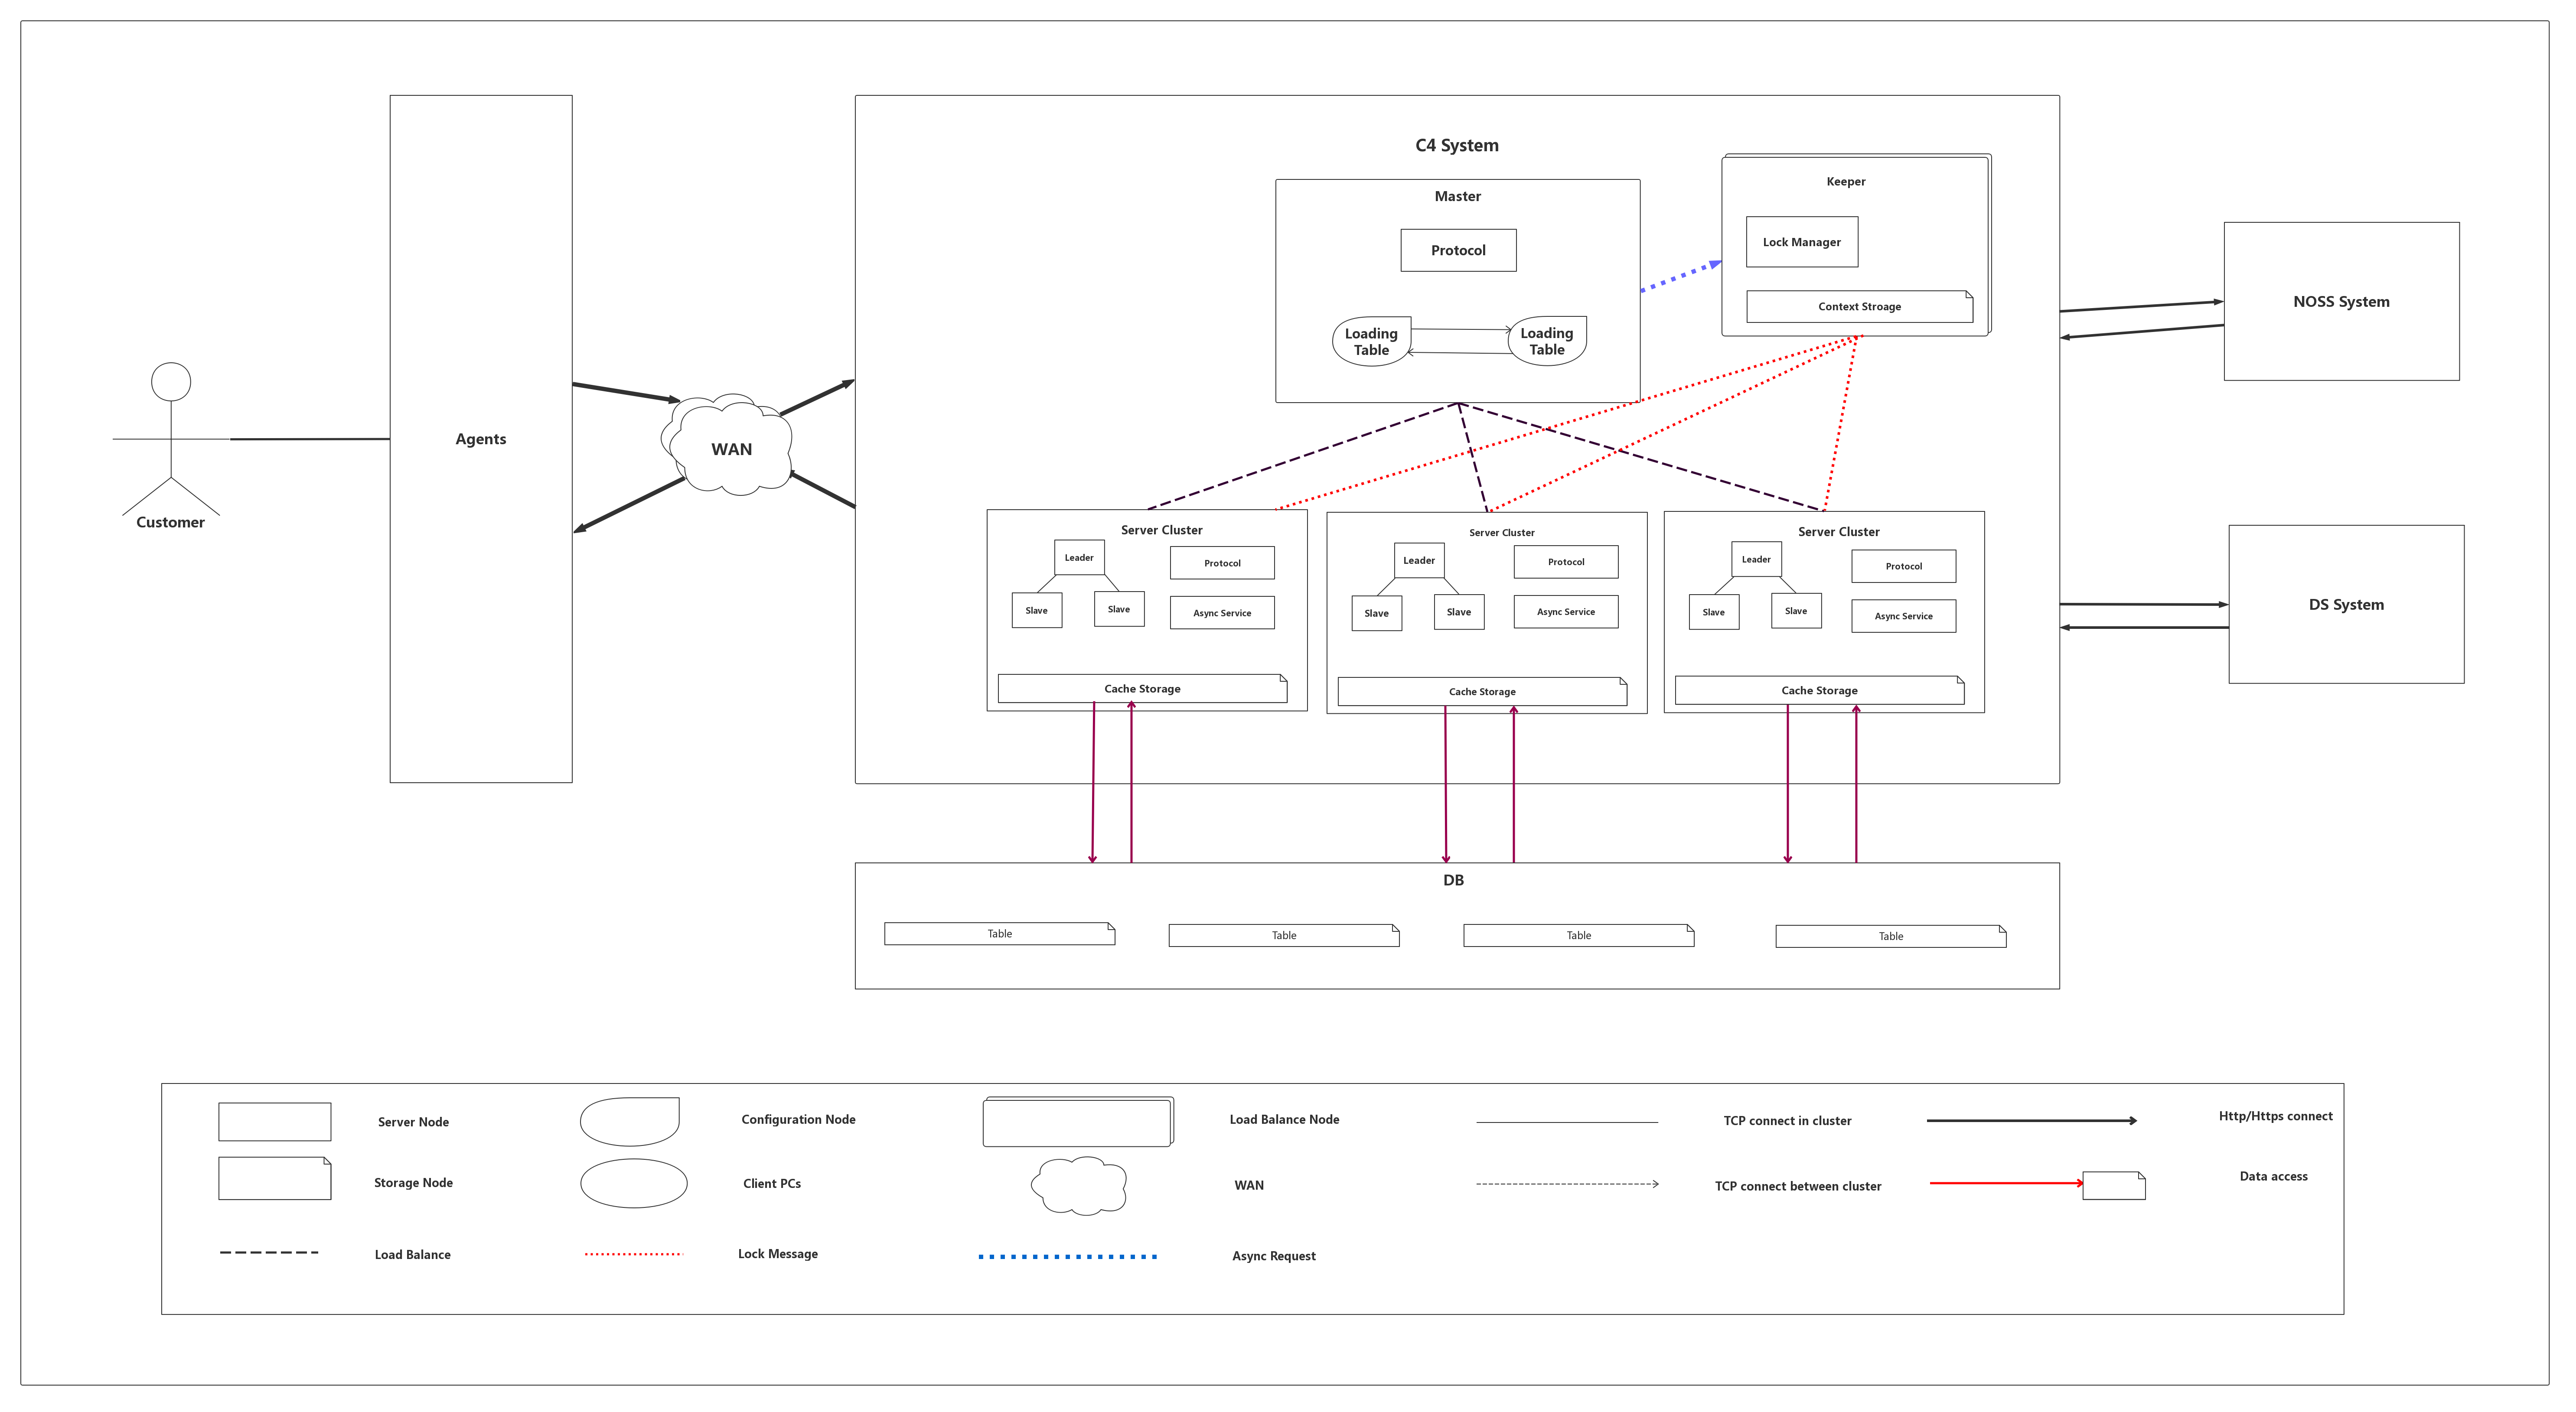
\includegraphics[scale=0.05]{decom_section2.png}
			\end{center}
			\paragraph{Section 4: Variability Guide}
			The decomposition view represents the template module in the C4 system , and to exercise the variation points , you are recommended to run the server node. With the sync-request (like fetching user basic information , setting up a new session)  and async-request (conflict between the different sessions) , you could catch the key points in the master.
			\paragraph{Section 5: Rationale}
			The PC agents communicate with C4 system across the WAN. 
			Master node stands for the whole manager of C4 system . That is ,  the master node uses the loading table to temporarily record the load status of all subordinate slave server clusters, and can timely alarm and resource reallocation. The master node also contains a protocol subnode, which is mainly used to help the master node process user requests. After the agents send the request, they will first be parsed by the master node to inform the agents of the required service node location, and then the agents will send the request to the target server.	
			The keeper is responsible for asynchronous event processing and session saving between server nodes. Use Lock Manager to allocate locks and save contexts through context storage.
			The server node is mainly responsible for periodically reporting heart beat status to the master node, and can perform hot backup between nodes. Please note that one server node here is also a cluster. In our design, one cluster is responsible for a certain range. The service (similar to the microservices architecture), and the leader is elected by the vote inside the cluster to perform resource scheduling and service allocation to the subordinate slave. In addition, the server node also supports the processing of the protocol and async service. Responsible for the interaction of the NOSS and DS systems. The cache storage is responsible for the caching of the external DB system. Since each business request will design a query of more than a dozen data tables, considering the time loss of the cascaded query, we use the cache mechanism to The query result is cached inside the server.

		\subsubsection{Shared-Data View} 
			\paragraph{Section 1: The Primary Presentation}
			\begin{center}
			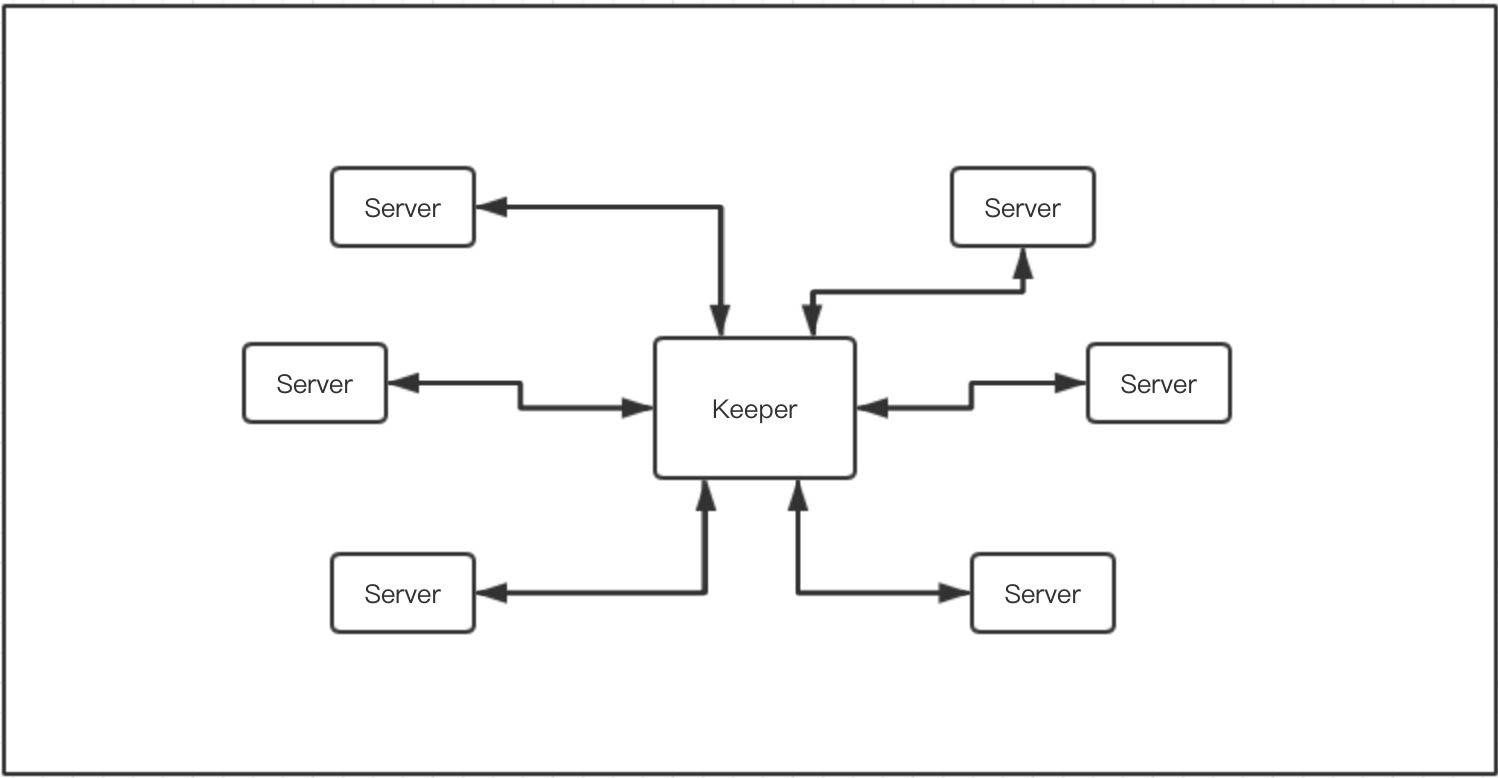
\includegraphics[scale=0.3]{share.png}
			\end{center}
			\paragraph{Section 2: The Element Catalog}
			\subparagraph{Elements and their properties}
			\begin{itemize}
			\item{Keeper} The keeper is a data storage center which holds the shared data.
			\item{Server} The server is an entity which stores and fetches data from the Keeper. For example, when a customer temporarily terminates the process, server should save the context for a future reference.
			\end{itemize}
			\subparagraph{Relations and their properties}
			During the fetching process, there may not exist the record, so there should be an exception. Also, in the saving process, to those records that already existed, saving process should be an update to the old version.
			\subparagraph{Element interfaces}
			The Keeper should provide the find and insert interfaces to the servers.
			\subparagraph{Element behavior}
			The servers save and fetch the data from the Keeper.
			\paragraph{Section 3: Context Diagram}
			\begin{center}
			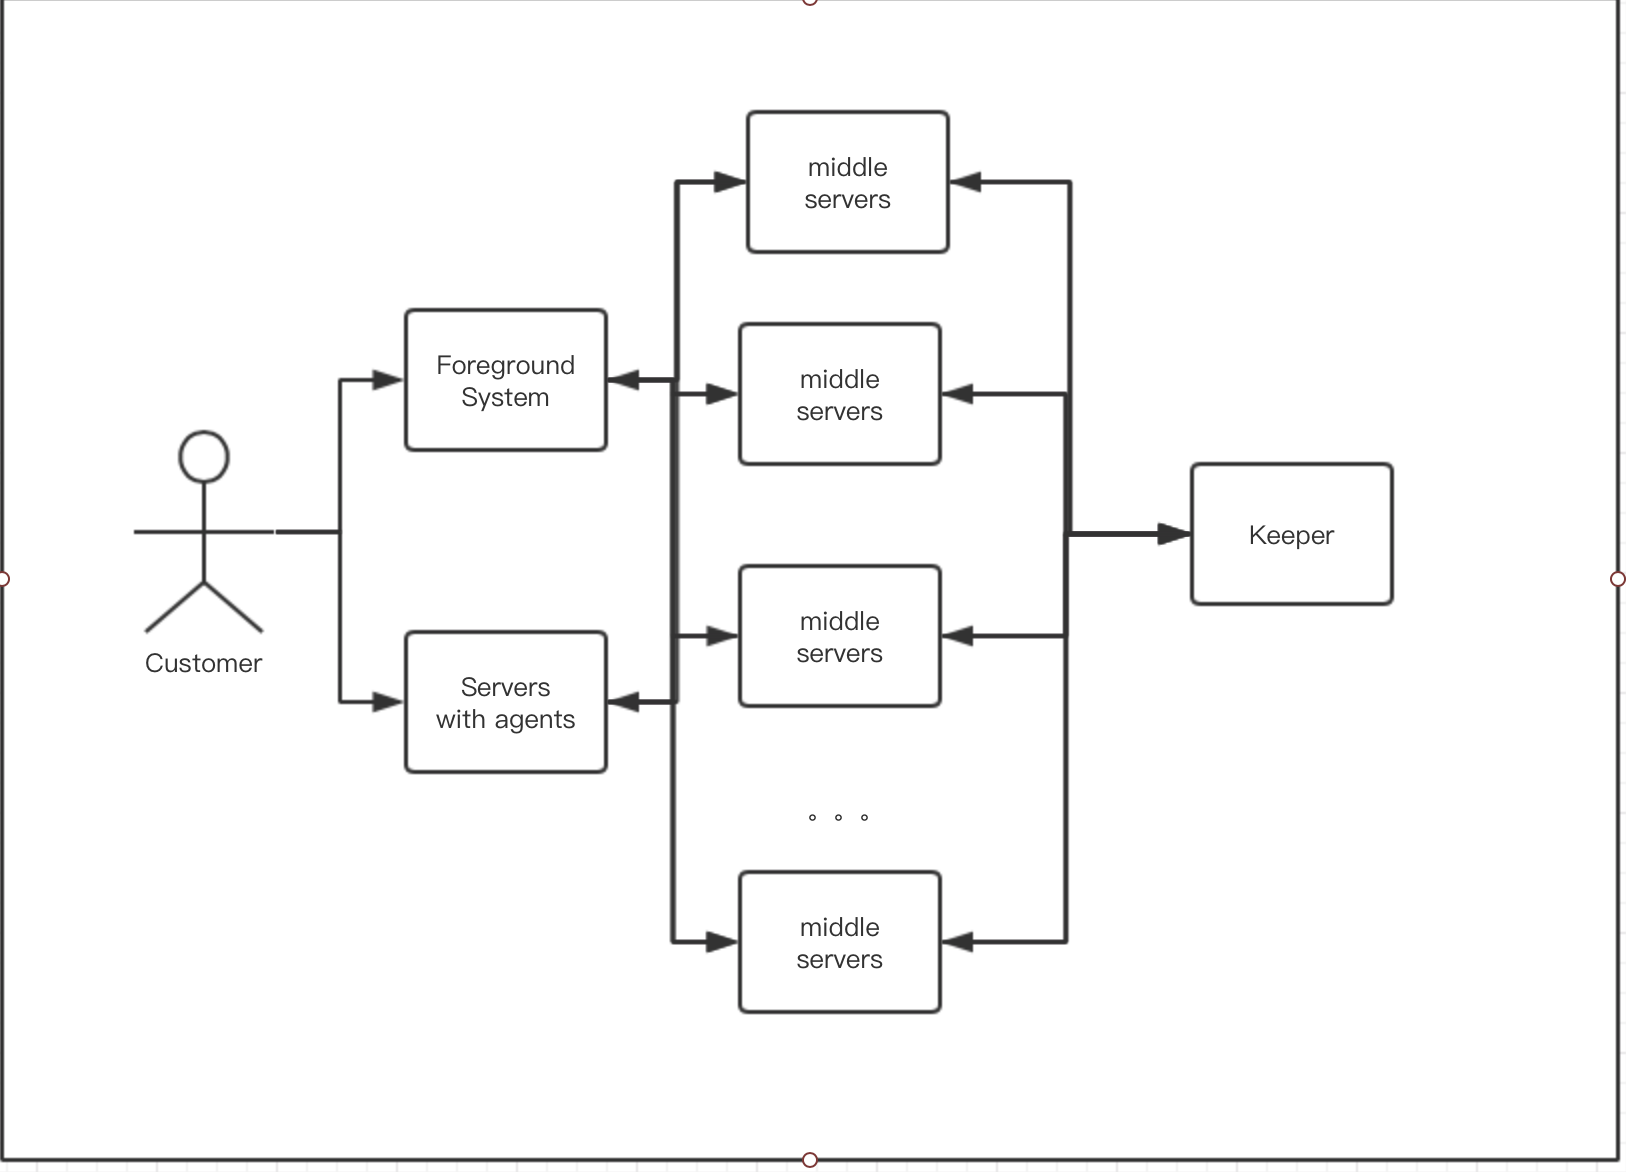
\includegraphics[scale=0.3]{share2.png}
			\end{center}
			\paragraph{Section 4: Variability Guide}
			Because the data storage is not the only responsibility keeper takes, so in the future, it may be  divided into several more specific components, that is to say, the keeper in this view may be changed to a data repository or other data center.
			\paragraph{Section 5: Rationale}
			The design problem came from the requirement "A customer can be interrupted (for technical reasons, for example) or suspended by the customer or the representative ... In any case, C4 has to manage the context that persists and can be recalled."
			In order to do this, there should be a mechanism that stores and fetches the context. There are several options. For example, we can save the information in the agent's PC, or save in the DB provided by the third party. But both of them are infeasible. There is no persistent data caching on the agent workstations, and DB may not be changed since it is provided by the third party. So finally, we choose to save the information in the Keeper, as it is also used to synchronize the event and resolve the conflict as mentioned in the sections before.

		\subsubsection{Deployment View} 
			\paragraph{Section 1: The Primary Presentation}
			\begin{center}
			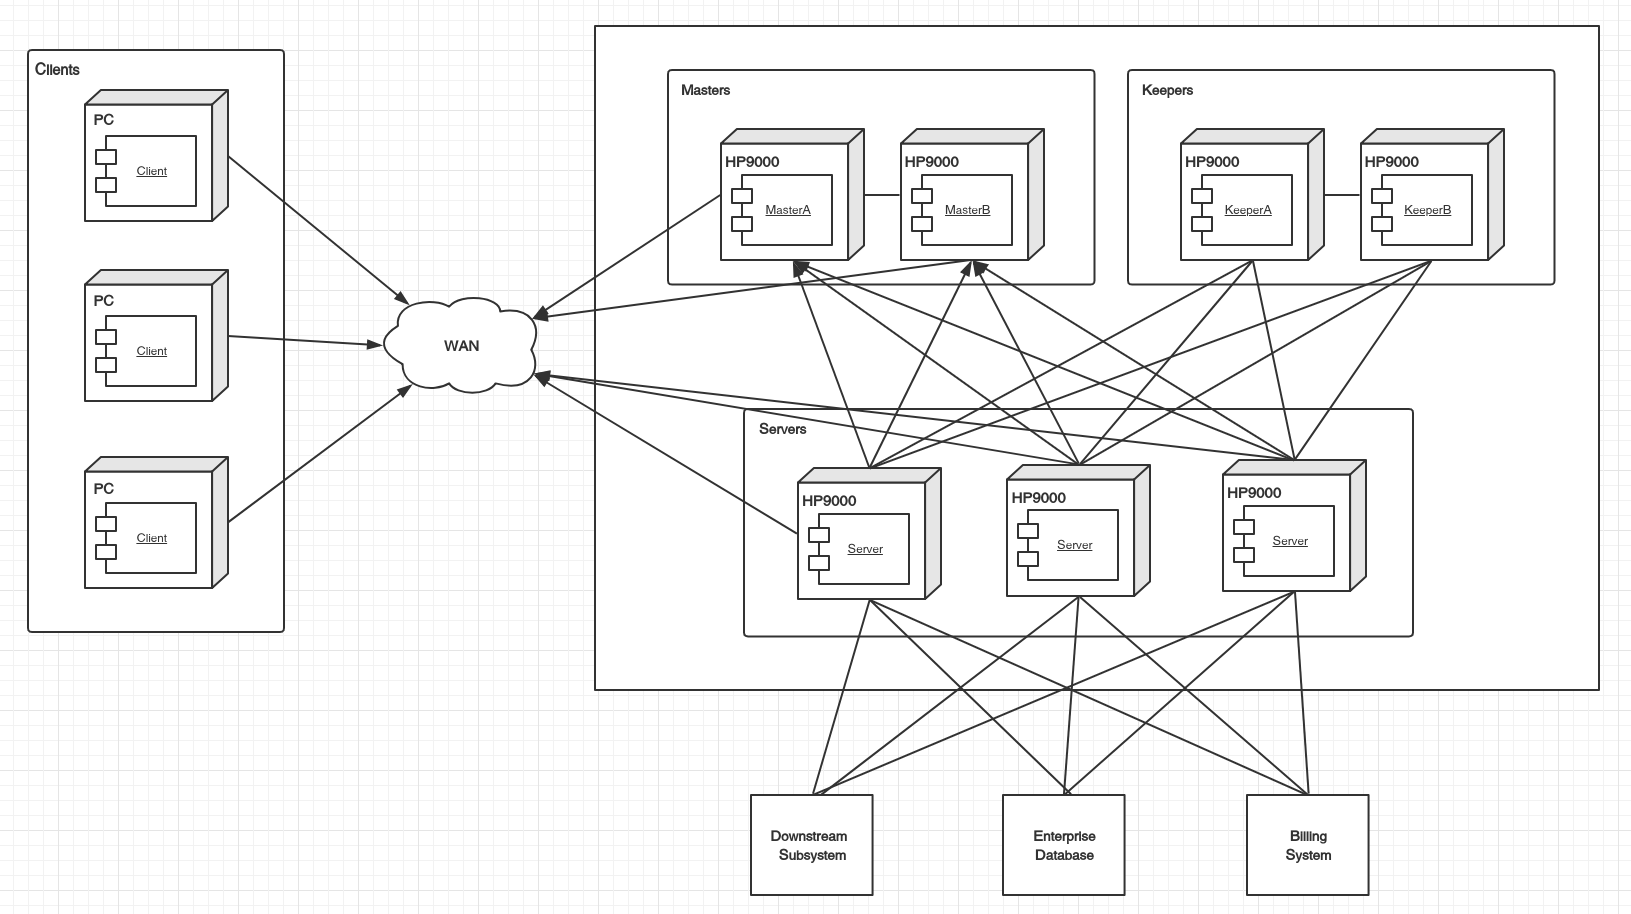
\includegraphics[scale=0.25]{deployment1.png}
			\end{center}
			\paragraph{Section 2: The Element Catalog}
			\subparagraph{Elements and their properties}
			\begin{itemize}
			\item{Client} The element Clients are deployed in the physical nodes placed in the office, which is running on Windows 10 PC.
			\item{Master} The master node of server cluster, providing functionalities such as load balancing, service registration, and service management. The master node is deployed independently to two HP9000 servers through dual hot standby mode.
			\item{Server} Server is the node that provides business service processing capabilities in the server cluster and is deployed on multiple HP9000 servers. These server nodes are redundant nodes and provide the same business service processing functionality.
			\item{Keeper} Distributed service coordination node, providing distributed locks and service processing context storage for server node cluster.
			\end{itemize}
			\subparagraph{Relations and their properties}
			\begin{itemize}
			\item{Client} Processing the business by communicating
			 with the server cluster through the WAN
			\item{Master} Clients will request the Master to obtain services list and Master will return a suitable services list for Clients based on the current load.
			\item{Server} The actual request of Clients is directly performed with the Server, not Master; when the Server node starts, it will register the service with the Master node, keep connection with Master node during the normal service provision, and report the load status and other information to Master node; During the business processing, the Server nodes will communicate with other systems outside (including downstream subsystems, enterprise databases, billing systems, NOSS, etc.) when necessary.
			\item{Keeper} The Server node will obtain or release the lock from Keeper; when involving business interruption or recovery, the Server node will also save or obtain the business context from Keeper.
			\end{itemize}
			\subparagraph{Element interfaces}
			\begin{itemize}
			\item{Client} End user interaction interface
			\item{Master} Service registration interface; service list acquisition interface; load information collection interface
			\item{Server} All business function interface; synchronous/asynchronous communication interface with external system
			\item{Keeper} Read/Write interface of business context information; lock service interface
			\end{itemize}
			\subparagraph{Element behavior}
			\begin{itemize}
			\item{Client} Respond to end user interaction
			\item{Master} In response to the Client's service list obtaining request, Master will generate an appropriate service list and returns according to the current cluster load situation and the predefined load balancing policy; Collecting periodic load information reports from Server nodes; If load information report of a Server node is not received within the certain period, the Server node is considered to be failed, and will be removed from the service list; Accept and process service registration requests from eht new Server nodes			
			\item{Server} Respond to Clients' business requests; Periodically processing asynchronous responses from external systems  in the message queue; When Clients request to interrupt the current business, the Server will save the current business context in Keeper, and when Clients request to restore the current business, Server obtains the stored context information from the Keeper and returns it; For each Client's business, Server will request Keeper to lock or release lock of related system resources 			
			\item{Keeper} Response to Servers' lock service request according to the current resources lock situation; Response to Servers' context read and write requests			
			\end{itemize}
			\paragraph{Section 3: Context Diagram}
			\begin{center}
			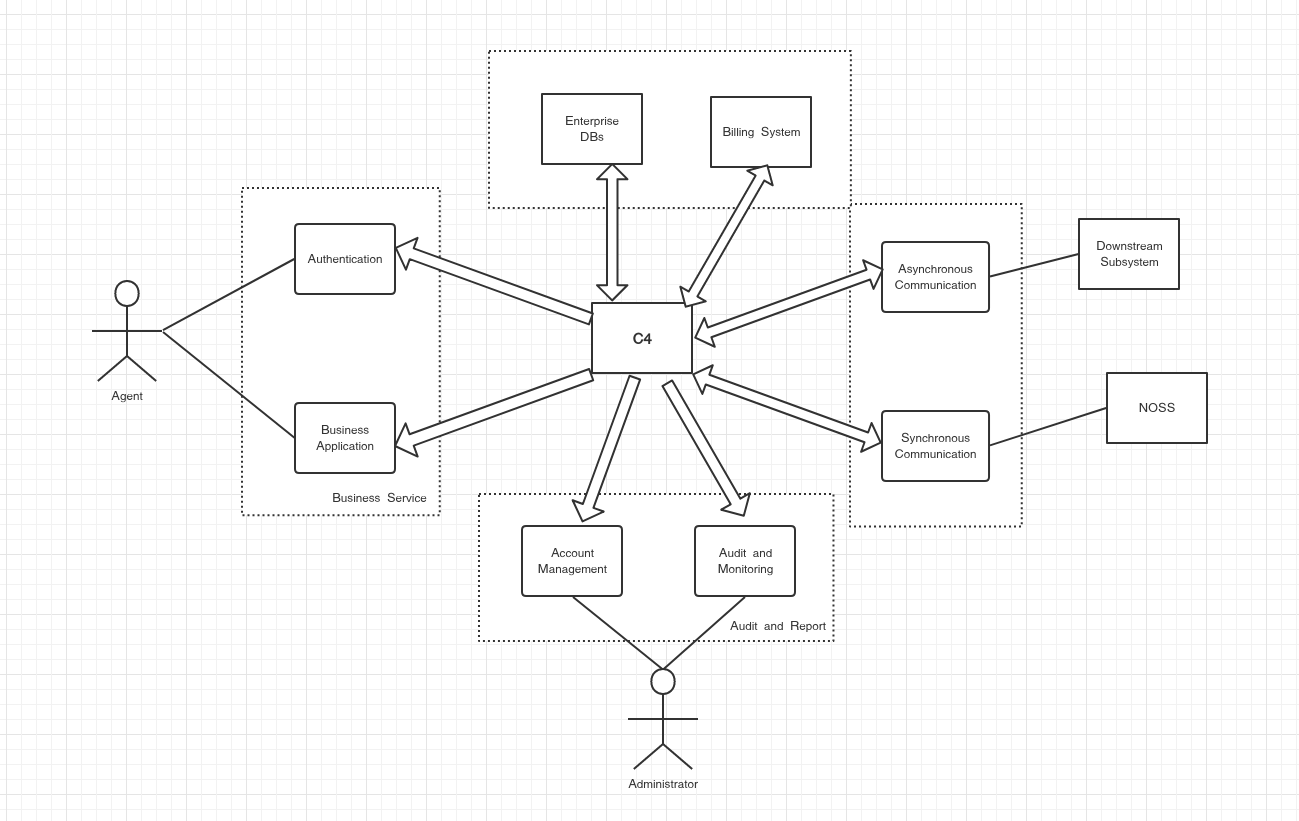
\includegraphics[scale=0.3]{deployment2.png}
			\end{center}
			\paragraph{Section 4: Variability Guide}
			With the growth of business in the future, the number of office agents will increase, so the number of Client nodes that need to be deployed will also increase. In order to cope with the larger work load, the Server nodes will introduce more deployment nodes accordingly.
			\paragraph{Section 5: Rationale}
			Because of the high availability requirement of the system, the system needs to respond to the failure of the Server nodes through redundancy (including Client nodes and Server nodes). Secondly, in order to coordinate the management of distributed Server node cluster, we introduce the Master node to implement service registration and service management, and in order to solve the single point failure, Master nodes adopt the scheme of dual-system hot standby and physical node independent deployment.\\
			Since the concurrent tasks in the normal service processing may cause problems such as configuration requests conflicts and system resource conflicts, and the requirement of saving the interrupted business context, the system needs to ensure data consistency under distributed clusters.Therefore, we introduces Keeper to provide the functionality of distributed lock, and in order to solve the problem of single point failure, Keeper nodes also adopt cluster mode and independent physical node deployment.

	\subsection{Mapping Between Views}
		\paragraph{Section 1: Mapping Selection}
		After designing the first three views, we found that the deployment view and the decomposition view are very similar, so we plan to measure and show the relationship between them.
		\paragraph{Section 2: Mapping Graph}
		\begin{center}
			\begin{table}[!htb]
			\begin{tabular}{ccc}
			\toprule  
			Element in Deployment view & Element in Decomposition view\\
			\midrule 
			Masters		& Protocol,\\
						& Loading Table\\
			Keepers		& Lock Manager,\\
						& Context Storage\\
			Servers		& Leader,\\
						& Slave,\\
						& Protocol,\\
						& Async Service,\\
						& Cache Storage\\
			Clients		& PCs / Agents\\
			\bottomrule
			\end{tabular}
			\caption{Mapping Graph}
			\end{table}
		\end{center}
		\paragraph{Section 3: Mapping Description}
		It is not difficult to see that the two views (Deployment and Decomposition) of the C4 system\\
		are almost identical at the cluster level, and all adopt the basic Master-Slave architecture mode. \\
		On a more granular level, the Masters implementation adopts the Protocol.\\
		And the implementation of the Keeping Table; keepers are implemented by Lock Manager and Context Storage, so the keeper has the coordination function; \\
		the working cluster Servers are implemented by Leader, Slave, Protocol, Async Service, Cache Storage, and external systems and agents. Interact. \\
		In addition, Clients are implemented by multiple PC physical machines.\\

	\subsection{Rationale}
	Explain what decision we have made in our views.

	\subsection{Directory}

	\begin{itemize}
		\item{Client} Respond to end user interaction
		\item{Master} In response to the Client's service list obtaining request, Master will generate an appropriate service list and returns according to the current cluster load situation and the predefined load balancing policy; Collecting periodic load information reports from Server nodes; If load information report of a Server node is not received within the certain period, the Server node is considered to be failed, and will be removed from the service list; Accept and process service registration requests from eht new Server nodes			
		\item{Server} Respond to Clients' business requests; Periodically processing asynchronous responses from external systems  in the message queue; When Clients request to interrupt the current business, the Server will save the current business context in Keeper, and when Clients request to restore the current business, Server obtains the stored context information from the Keeper and returns it; For each Client's business, Server will request Keeper to lock or release lock of related system resources 			
		\item{Keeper} Response to Servers' lock service request according to the current resources lock situation; Response to Servers' context read and write requests			
		\item{protocol} Mainly used to help the master node process user requests. After the agents send the request
		\item{lockManager} Allocate locks and save contexts through context storage
		\item{Cache} When the response messages of other systems reach the system, they will be cached in the system
		\item{Async Service} Receive the async message and rearrange the message queue to avoid the message conflict.
		\item{Loading Table} Store the sub server loaction and ready to return back to agents; Used for load balance.
	\end{itemize}

	\section{Personal Remarks}
	\subsection{Statement of ...}
	\subsection{Statement of Peihong Chen}
	\paragraph{1: ADD experience}
	ADD is a practical software architecture design method, the overall design is a top-down progressive refinement, and after several rounds of iteration, it makes the software designers to progressively deeper understanding on the system. Each iteration is independent and interrelated, because each round of iteration will only focused on one or a few specific quality attributes, which can avoid unnecessary interference; In addition, subsequent iterations can also conduct a deeper analysis based on the previous iteration, so there is some relationship between iterations. The cycle continues until the architectural elements and responsibilities of the entire system are clear.
	\paragraph{2: Contribution}
	During this assignment, in the early stage team members participated in functional and non-functional requirements analysis and ASRs identification. Then, in all the four iterations, team members discussed together, exchanged opinions and made decisions on some vague points. My main contributions are scalability, interoperability and data consistency of stimulation corresponding sequence, the second iteration of service recovery (including quick restart, transparent to PC, and data recovery) and resources in the third iteration consistency (including detecting data conflicts, restore data inconsistency, and prevention of data). In addition, in the documentation process, my main contribution is  writing the deployment view and working with other team members to complete the cross-view.

	\subsection{Statement of Shaoxun Zeng}
	\paragraph{1: ADD experience}
	I feel it is difficult to narrow down the focuses. For example, in the ADD second iteration, we choose the “broker node” to break down. And we brainstormed many ideas, but when we came to the “Design Concerns” section, it is difficult to summerize them into several main categories.
Also, figuring out the tactics used to solve the architetural requirements is a big deal to me since we lack the development experience. I could only do my best to “imagine” the real situations combined with the information gathered from the Internet.
In a nutshell, it is useful to follow these steps. In the last phase, when I put all the parts together, I find it is natural to reach the final result with our refinement, which is not such an obvious result from the first glance of the requirement document.
	\paragraph{2: Contribution}
	During the disccusion, I participated in the whole process.
	More specificly, I wrote some scenarios of the ASR, participated in the all iterations of ADD, gave out some tactics and requirement specifications, documented the Shared-Data View.
	And also, I think I pushed the whole process during the disccusion. For example, when we stuck in the brainstorming, I suggested to move on and came back to this point a fewer minutes later. 
	And also, since we use the latex for formating, I do a lot of works about the formating.

	\subsection{Statement of Fangming Lu}
	\paragraph{1: ADD experience}
		In the process of using ADD, special attention should be paid to the selection of ASR, \\
	because it will affect the final result. The initial ASR needs to be given in detail, taking into account the key points in the demand. \\
	For example, the same in this C4 system. Asynchronous problems, conflict resolution problems, what kind of effects are needed to be realized at the beginning, \\
	and can be well targeted for subsequent tactics.\\
	In addition, in the selection process of the view, the factors that need to be considered are beyond the expectations of the beginning. \\
	In order to get a more objective view selection, each participant in the process from product demand to release is evaluated for importance.\\
	\paragraph{2: Contribution}
	Participated in each iteration process, participated in the planning of the master service registration function, \\
	imitated the typical master-slave architecture, and gave the node design, resource allocation, resource recovery, horizontal expansion of the architectural design. \\
	Also responsible for integrity , reliability, ease of use of the Scenario design, and gives the five section design of the decomposition view\\

	\subsection{Statement of ...}
\end{document}